\label{section:vertex-area-chapter}
This section shows alternative methods to extend the idea of flat shading from triangles to vertices and edges. The idea of flat shading is to draw all the pixels of a triangle with the same colour. The extension of this approach is to split the surface of the triangle mesh likewise into regions around vertices and edges and draw all pixels in these regions with the same colour (Fig. \ref{fig:vertex-area}), thus visualizing data given at the vertices or edges of the mesh in a piecewise constant, not necessarily continuous way, resembling the classical triangle flat shading. The aforementioned regions can easily be defined using barycentric coordinates and a simple GPU fragment program (Fig. \ref{fig:max-diagram}) can be used to find out for each pixel to which region is belongs and which colour it should be painted with.

%%%%%%%%%%%%%


\begin{figure}[h]
    \centering
    \minipage[b]{.5\linewidth}
    \centering
    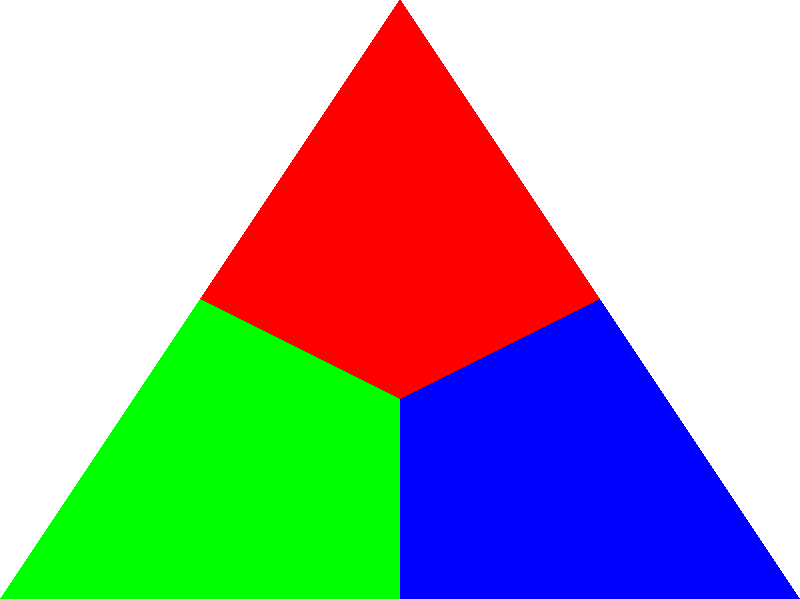
\includegraphics[scale=0.15]{images/max.png}
    \caption{Max diagram}\label{fig:max-diagram}
    \endminipage\hfill
    \minipage[b]{.5\linewidth}
    \centering
    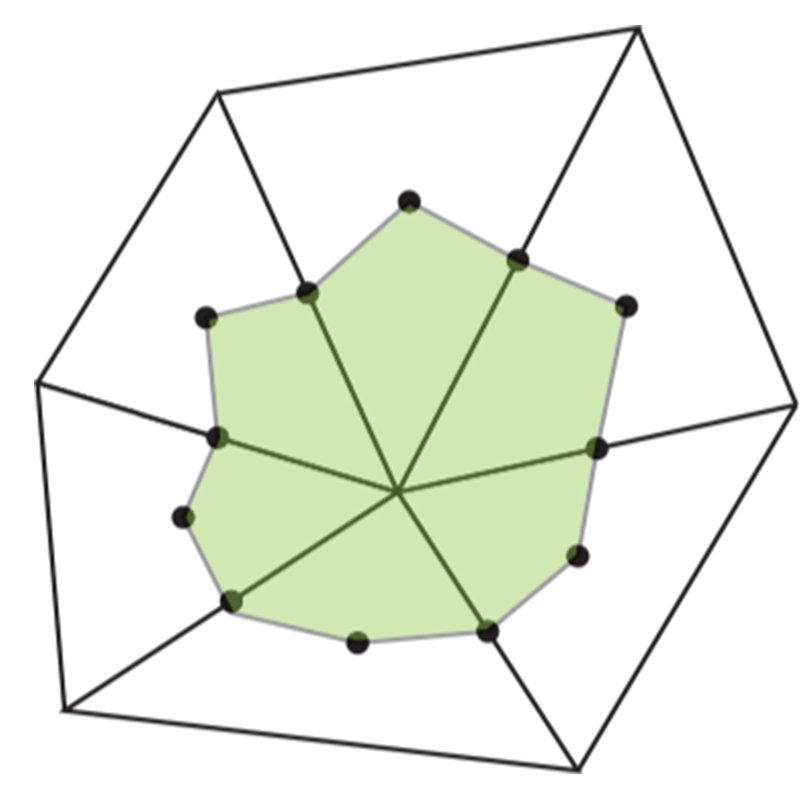
\includegraphics[scale=0.15]{images/vertex-area.png}
    \caption{Region around a vertex}\label{fig:vertex-area}
    \endminipage
\end{figure}

%%%%%%%%%%%%%

\subsection{Max diagram - Vertex based area} \label{section:max-diagram}
Passing barycentric coordinates to the \textit{fragment shader} will clearly demonstrate that we can get different results from the classic color interpolation.\cite{WEBSITE:redbloggames}
%----------
There are different approaches to color interpolation focusing on the distance from vertices. For each point in a triangle, we can easily determine its closest vertex, which we use as a cue for coloring.
A different approach from interpolating, can be found coloring vertex areas based on the minimum barycentric coordinate.
The color is given by the region farthest from a vertex (Fig. \ref{fig:max-diagram}, Pseudocode \ref{appendix:max-diagram}).

%%%%%%%%%%%%%

\subsection{Flat shading per vertex} \label{section:extend-flat-shading-lighting}
An extension of \textit{flat shading} would be to have each vertex area to be in one constant color. This color can be taken using the normal at the vertex and the vertex position.
The color will then be computed as in \textit{Gouraud shading}.
The idea is to compute the color per vertex but instead of linearly interpolated it in each triangle (as \textit{Gouraud shading} does) we color regions around a vertex with that constant color (using the GPU fragment program: max diagram \ref{section:max-diagram}).
To implement it, the barycentric coordinates, the vertex color, the normal at the vertex and the lighting calculations must be passed to the \textit{fragment shader}.
We want to avoid an automatic interpolation of colors, in order to return the resulting color using the \textit{max diagram}, we have used a \textit{Geometry shader} that have access to all three vertex colors in \textit{fragment shader}. (Pseudocodes: \ref{appendix:vs-flat-shading-lighting}, \ref{appendix:gs-flat-shading-lighting}, \ref{appendix:fs-flat-shading-lighting})

\begin{figure}[!h]
    \centering
    \minipage[b]{.3\linewidth}
    \centering
    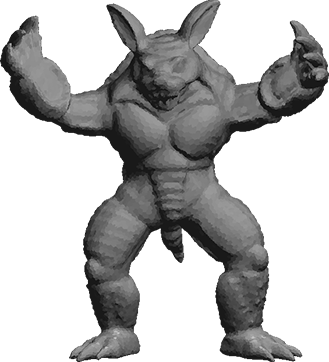
\includegraphics[scale=0.3]{images/armadillo-extendfs.png}
    \endminipage\hfill
    \minipage[b]{.3\linewidth}
    \centering
    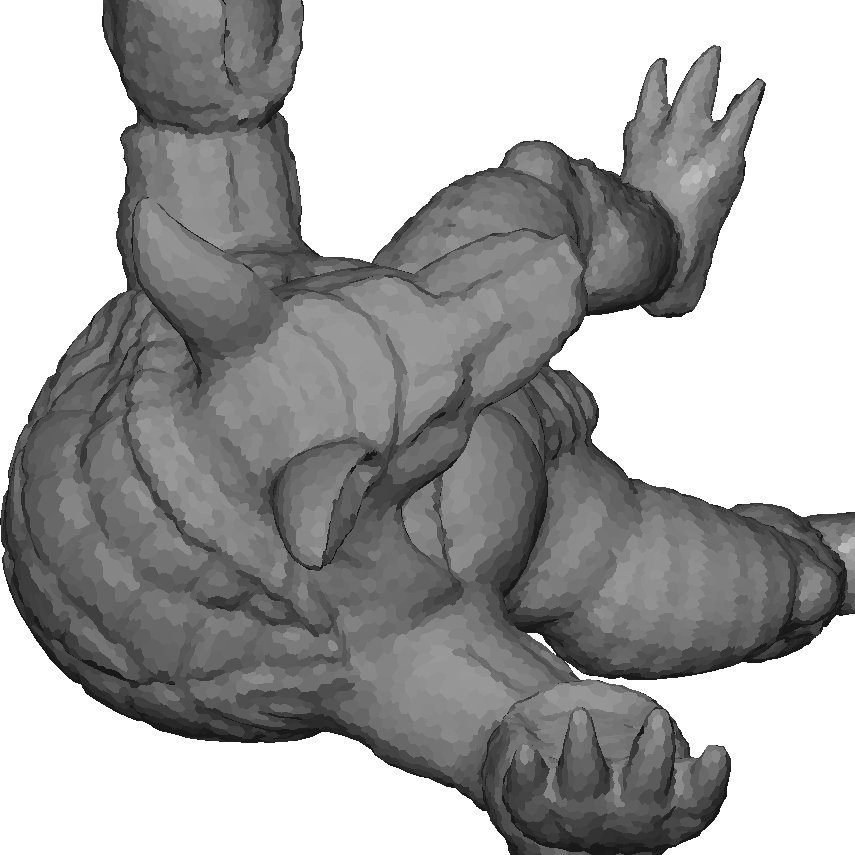
\includegraphics[scale=0.3]{images/armadillo-extendfs-1.png}
    \endminipage\hfill
    \minipage[b]{.3\linewidth}
    \centering
    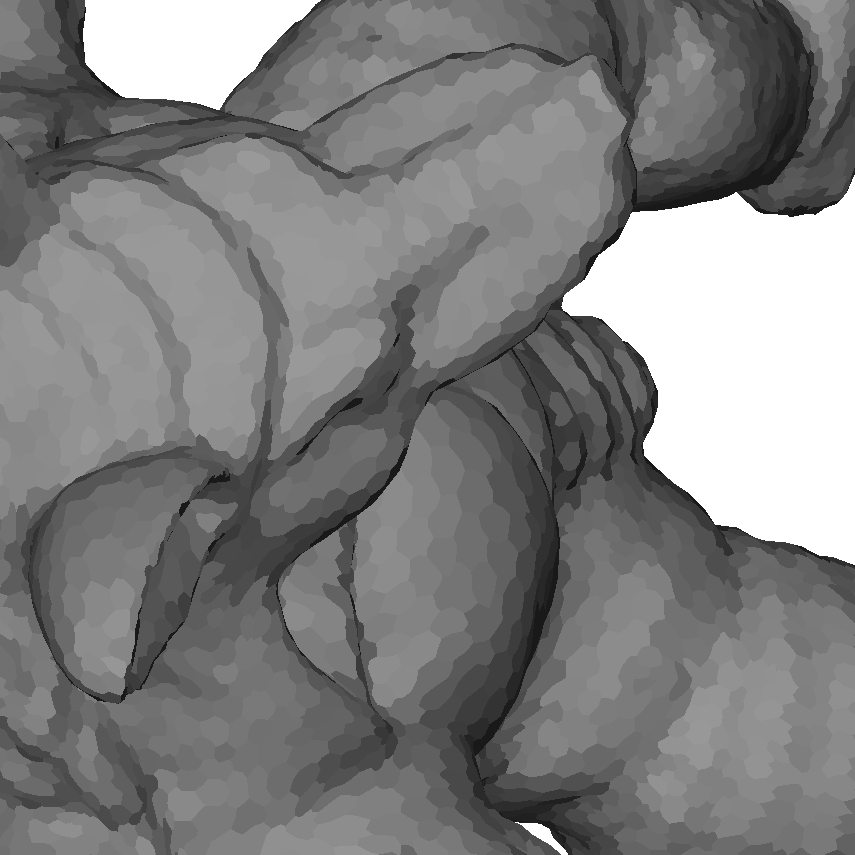
\includegraphics[scale=0.3]{images/armadillo-extendfs-2.png}
    \endminipage
    \caption{Flat shading per vertex}
\end{figure}


\subsubsection{Comparison}
\color{red}{TODO: add armadillo, horse, etc. images with these 3 effects (flat shading 1 and 2, gouraud shading)}
\color{black} %to remove after
\begin{figure}[!h]
    \centering
    \minipage[b]{.3\linewidth}
    \centering
    % \includegraphics[scale=0.15]{images/.png}
    \caption{Flat shading per triangle}\label{fig:flat-shading-triangle}
    \endminipage\hfill
    \minipage[b]{.3\linewidth}
    \centering
    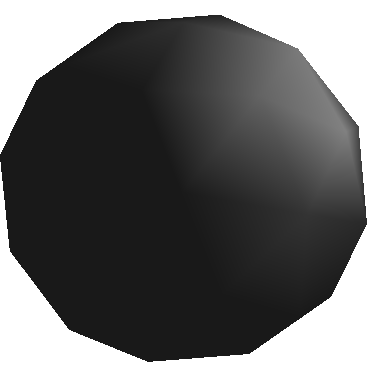
\includegraphics[scale=0.5]{images/gouraudshading.png}
    \caption{Gouraud shading per triangle}\label{fig:gouraud-shading}
    \endminipage\hfill
    \minipage[b]{.3\linewidth}
    \centering
    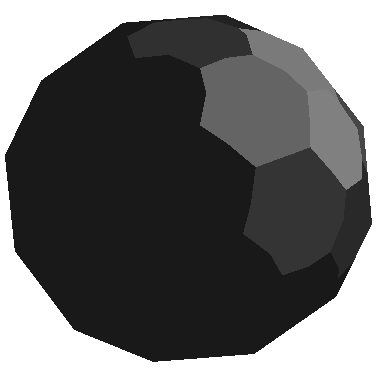
\includegraphics[scale=0.5]{images/extentflatshading.png}
    \caption{Flat shading per vertex}\label{fig:flat-shading-vertex}
    \endminipage
\end{figure}

%%%
\subsection{Gaussian curvature}
\label{section:vertex-area-gaussian-curvature}
Another interesting alternative data visualization technique is to compute the \textit{Gaussian curvature} per vertex. That can be done summing up, for each vertex, angles at this vertex with adjacent triangles and then subtracting this value to $2\pi$.
After having obtained this value, called \textit{angle defect} (Fig. \ref{fig:gc-angle}), we map linearly this value to a color range.
The resulting color will be the vertex flat shading visualisation of \textit{Gaussian curvature}.
$$K(V) = (2\pi - \sum_j \theta_j)/\mathcal{A}_{Mixed}$$
(See Section \ref{section:localaveraging} and \ref{section:gaussian-curvature-intro}).
%%
\begin{figure}[!h]
    \centering
    \minipage[b]{.5\linewidth}
    \centering
    \scalebox{0.65}{\begin{tikzpicture}
        \coordinate (J) at (3.1,2.9);
        \coordinate (circle) at (3.1,2.9);
        \node[anchor=south west,inner sep=0] at (0,0) {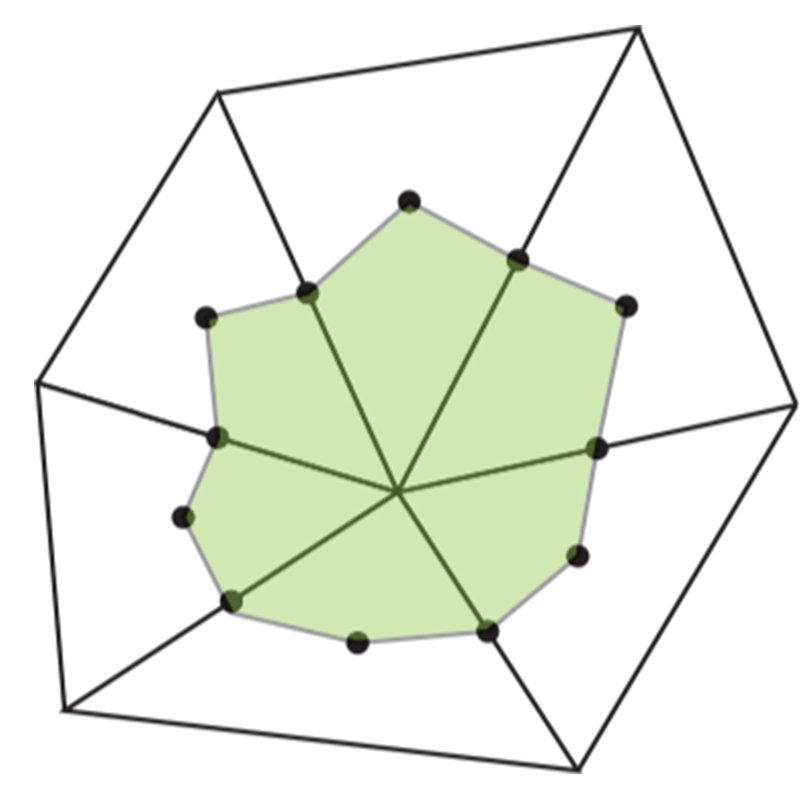
\includegraphics[scale=0.2]{images/vertex-area.png}};
        \draw (J) node [below left] {$j$};
        \filldraw (2.8, 2.2) circle (2pt);
        \begin{scope}[line width=0.4mm, line cap=round]
            \draw (3.2,1.7) arc (295:360:0.7cm) node[near start,right] {$\theta_j$};
        \end{scope}
    \end{tikzpicture}}
    \label{fig:gc-angle}
    \endminipage\hfill
    \minipage[b]{.5\linewidth}
    \centering
    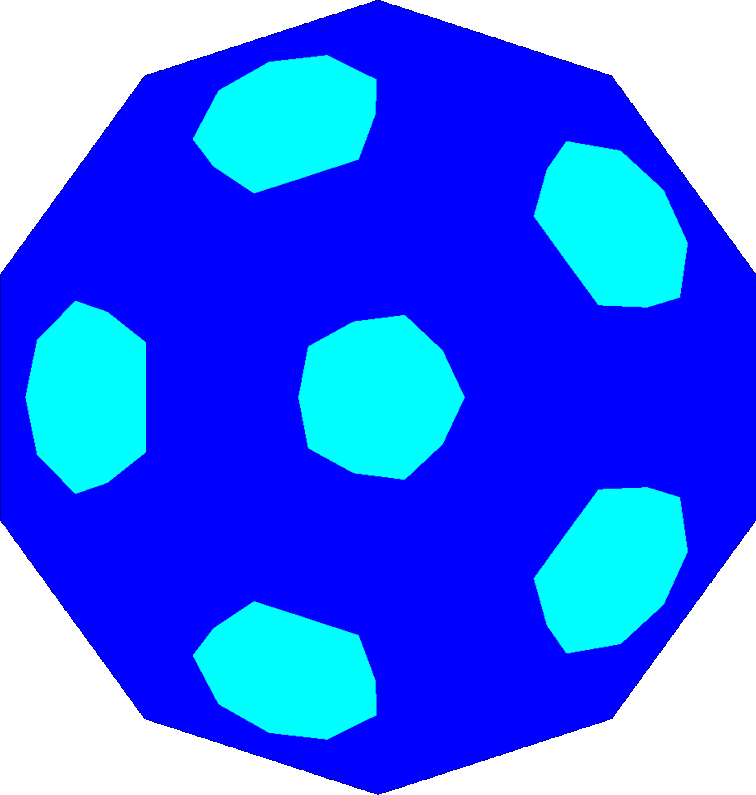
\includegraphics[scale=0.13]{images/gaussian-ball.png}
    \label{fig:gc-icosahedron}
    \endminipage
    \caption{On the left: angle defect is denoted with $\theta_j$. On the right: analysis that shows how constant vertex area should look on an icosahedron.}
\end{figure}
%%

%%%%%%%%

\subsection{Constant Gaussian curvature per vertex}
\textit{Constant Gaussian curvature per vertex} returns a constant color around each vertex (Fig. \ref{fig:gc-icosahedron}, Pseudocode \ref{appendix:vs-gaussiancurvature}). After having calculated the \textit{Gaussian curvature} per vertex, this value is mapped into a color range to get the curvature color (for example: green for flat surfaces). This process is made separately for each vertex of the triangle and after, using the technique explained above of max-diagram (See section \ref{section:max-diagram}) the final resulting constant color is returned.
\begin{figure}[!h]
    \centering
    \minipage[b]{.5\linewidth}
    \centering
    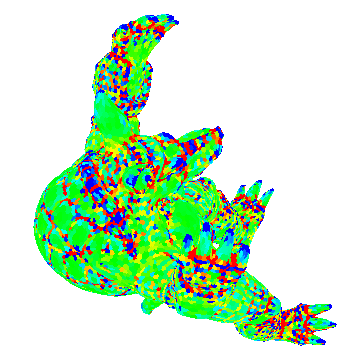
\includegraphics[scale=1.0]{images/gc-armadillo-top.png}
    \endminipage\hfill
    \minipage[b]{.5\linewidth}
    \centering
    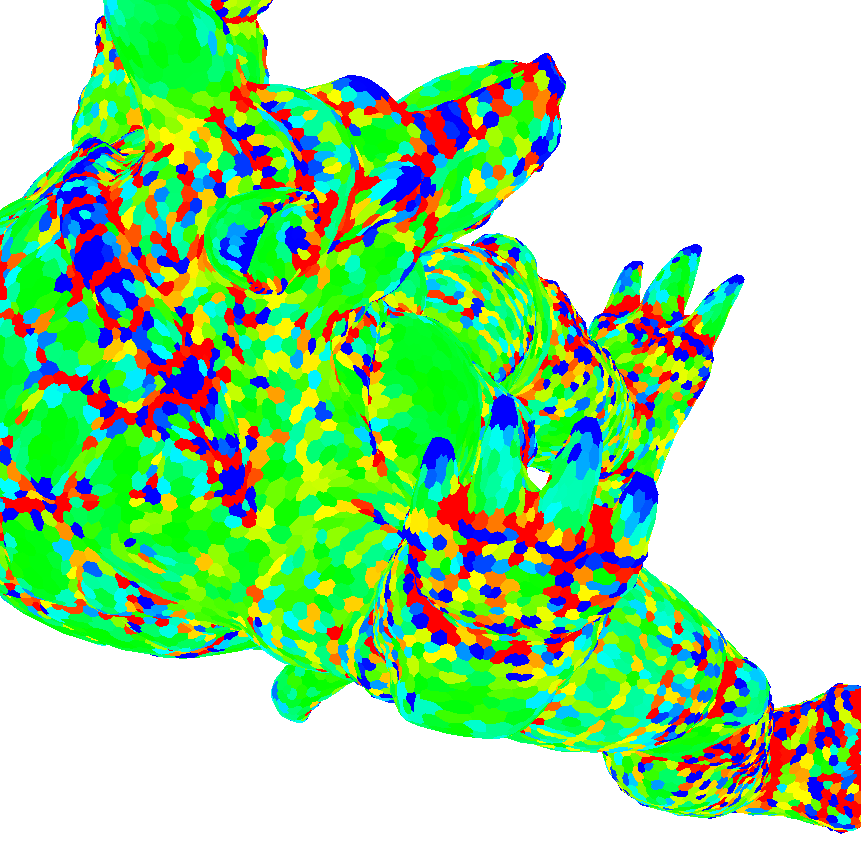
\includegraphics[scale=0.4]{images/gc-detail-armadillo-top.png}
    \endminipage
    \caption{Constant Gaussian curvature per vertex} \label{fig:gc-detail}
\end{figure}


\subsection{Gouraud Gaussian curvature}
\textit{Gouraud Gaussian curvature} returns an interpolated color per vertex. The idea is to calculate the \textit{Gaussian curvature} as explained above (mapping the color into a color range to get the corresponding color per vertex) but instead of returning the constant color using a max-diagram approach, we just return the interpolation of values obtained for each triangle.

\begin{figure}[!h]
    \centering
    \minipage[b]{.5\linewidth}
    \centering
    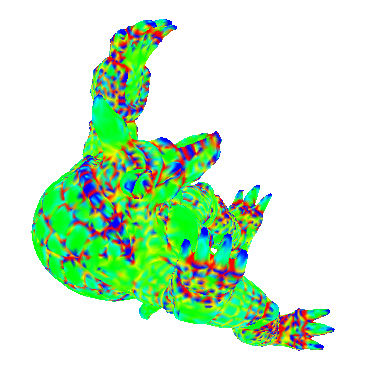
\includegraphics[scale=1.0]{images/gci-armadillo-top.png}
    \endminipage\hfill
    \minipage[b]{.5\linewidth}
    \centering
    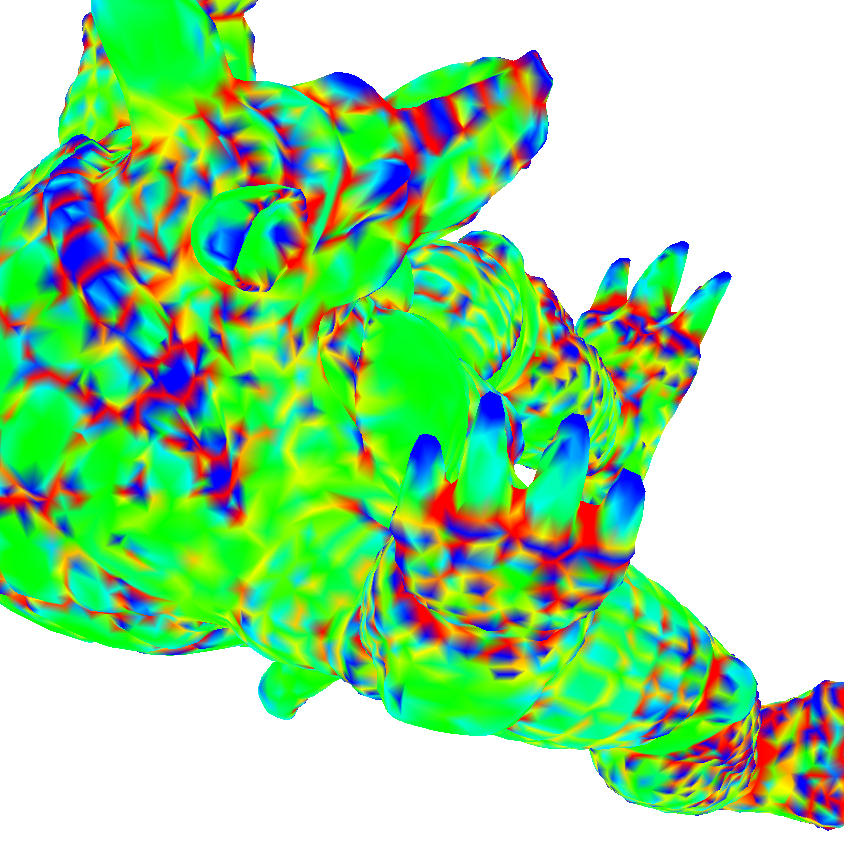
\includegraphics[scale=0.4]{images/gci-detail-armadillo-top.png}
    \endminipage
    \caption{Gouraud Gaussian curvature} \label{fig:gci-detail}
\end{figure}


\subsection{Evaluation and Comparison between constant Gaussian curvature per vertex and Gouraud Gaussian curvature}
We want now to compare the \textit{constant Gaussian curvature per vertex} (Fig. \ref{fig:gc-detail}) with the \textit{Gouraud Gaussian curvature} (Fig. \ref{fig:gci-detail}).
In Fig. \ref{fig:gc-detail} each vertex area is colored applying the method \textit{max diagram} described in the above section \ref{section:max-diagram}. Instead, in Fig. \ref{fig:gci-detail} the color is obtained with a linear interpolation.
Visualization of the principal curvatures of the model as colors from blue (highest values of curvature) to red (lower values of curvature) in Fig. \ref{fig:comparison-gc-gci} highlighs the geometry of meshes.
These changes of curvature, positive (blue), flat (green) and negative regions (red), better emphasizes the 3-dimensionality of the model.
\textit{Gouraud Gaussian curvature} is more smoothed that causes a loss of small details, this is particularly evident in armadillo's legs mesh. Instead, \textit{constant Gaussian curvature per vertex} generates sharped edges that less emphasizes the general lines of the model causing a small loss of 3-dimensionality.
\textit{Constant Gaussian curvature per vertex} better shows the muscle constrasts given a more detailed character to models.

\begin{figure}[!h]
    \centering
    \minipage[b]{.5\linewidth}
    \centering
    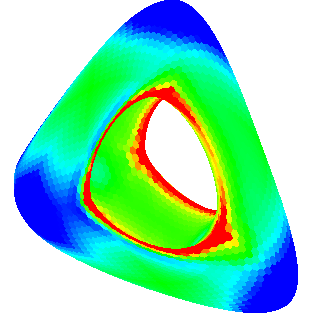
\includegraphics[scale=0.7]{images/gc-genus.png}
    \endminipage\hfill
    \minipage[b]{.5\linewidth}
    \centering
    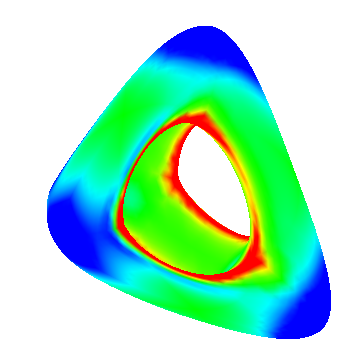
\includegraphics[scale=0.7]{images/gci-genus.png}
    \endminipage\hfill
    \minipage[b]{.5\linewidth}
    \centering
    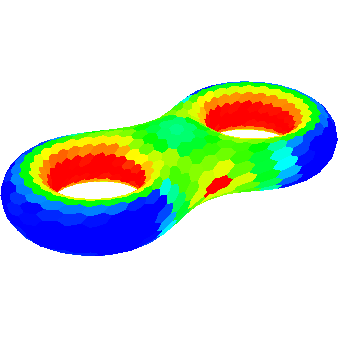
\includegraphics[scale=0.7]{images/gc-eight.png}
    \endminipage\hfill
    \minipage[b]{.5\linewidth}
    \centering
    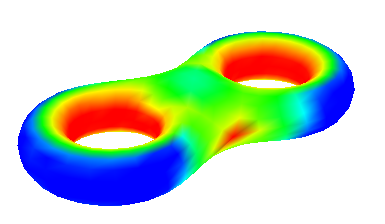
\includegraphics[scale=0.7]{images/gci-eight.png}
    \endminipage\hfill
    \minipage[b]{.5\linewidth}
    \centering
    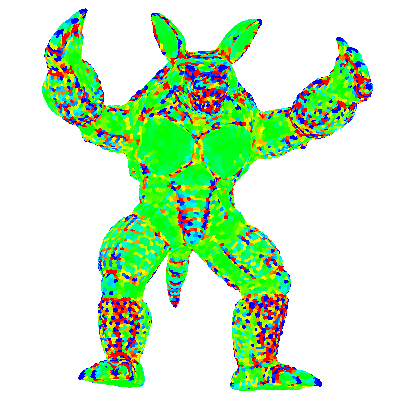
\includegraphics[scale=0.7]{images/gc-armadillo.png}
    \endminipage\hfill
    \minipage[b]{.5\linewidth}
    \centering
    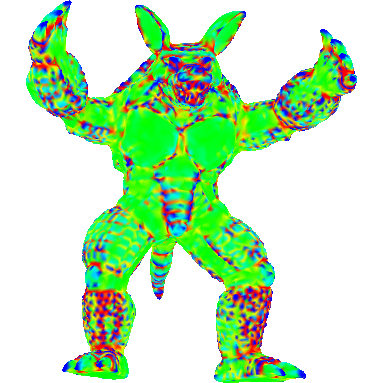
\includegraphics[scale=0.7]{images/gci-armadillo.png}
    \endminipage\hfill
    \minipage[b]{.5\linewidth}
    \centering
    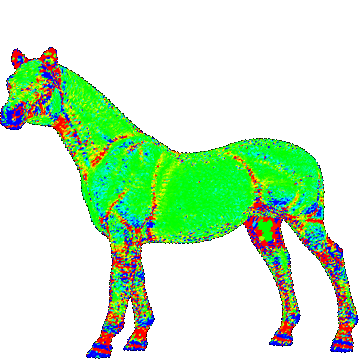
\includegraphics[scale=0.7]{images/gc-horse.png}
    \endminipage\hfill
    \minipage[b]{.5\linewidth}
    \centering
    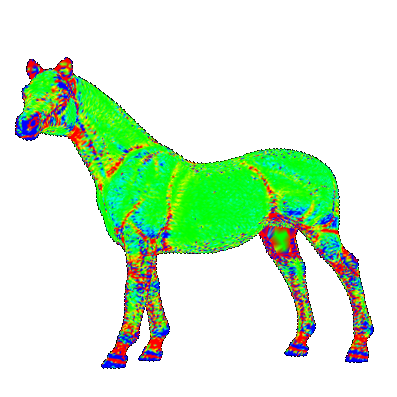
\includegraphics[scale=0.7]{images/gci-horse.png}
    \endminipage
    \caption{On the left: Constant Gaussian curvature per vertex. On the right: Gouraud Gaussian curvature.}
    \label{fig:comparison-gc-gci}
\end{figure}

